\section{Análisis estático automatizado de código}

	\subsection{Error nº1: Memory leak}

		\subsubsection{Origen/explicación del error detectado}
		
			\paragraph{}En la siguiente captura de pantalla se muestra el código fuente de la función \textit{modifica} de la clase plantilla \textit{lista\_sin} de nuestra aplicación.
			
			\begin{figure}[H]
				\centering
				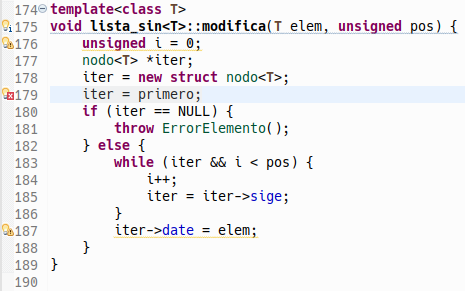
\includegraphics[scale=0.7]{img/captura42.png}
				\caption{Captura de pantalla de la función modifica}
				\label{captura42}
			\end{figure}
		
			\paragraph{}En la línea 179 cppchek nos indica que ha detectado un error de código, en concreto, se trata de un error de perdida de memoria para la variable \textit{iter}. Esto es debido a que en la línea 177 se declara la variable (la cual es un puntero a una estructura llamada \textit{nodo}, que hemos definido nosotros anteriormente en el mismo archivo), y en la línea 178 se inicializa con la palabra reservada \textit{new}. Al realizar esto anterior, hemos reservado memoria dinámica para la estructura y la hemos inicializado.
			
			\begin{figure}[H]
				\centering
				
\includegraphics[scale=0.38]{img/captura43.png}
				\caption{Detalle del mensaje de error de cppcheck}
				\label{captura43}
			\end{figure}
			
			\paragraph{}El error se origina cuando, en la línea 179, hacemos que la variable \textit{iter} (que es un puntero) apunte al atributo de la clase \textit{primero} sin liberar la memoria de la estructura con la que inicializamos anteriormente. Esto hace que la memoria que ocupa dicha estructura no se libere y que, por lo tanto, se produzca una pérdida de memoria. 
		
		\subsubsection{Corrección realizada para solventar el error}
		
			\paragraph{}La manera de resolver esta incidencia es de lo más trivial. Tan solo deberemos realizar la declaración de la variable y, acto seguido, asignarle la dirección de memoria del atributo de la clase \textit{primero}. A continuación, dejamos una captura de pantalla del estado de la función tras la resolución del error:
			
			\begin{figure}[H]
				\centering
				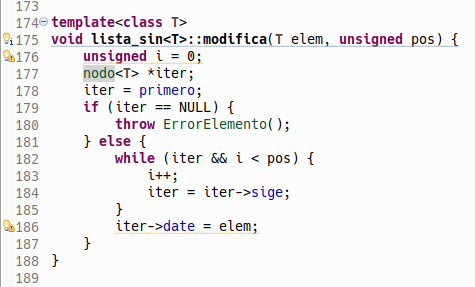
\includegraphics[scale=0.7]{img/captura44.png}
				\caption{Captura de pantalla de la función modifica tras la resolución del error}
				\label{captura44}
			\end{figure}
		
			\paragraph{nota:}Cabe destacar que también se podría haber resuelto este error realizando un $"delete$ $iter"$ antes de asignarle la dirección de memoria del atributo \textit{primero} pero en este hemos descartado esta opción ya que la estructura con la que se inicializa no se utiliza para nada y supondría la realización de operaciones innecesarias.
			
	\subsection{Error nº2: Memory leak}
	
		\subsubsection{Origen/explicación del error detectado}
		
			\paragraph{}En la siguiente captura de pantalla se muestra el código fuente de la función \textit{elimina\_dato} de la clase plantilla \textit{lista\_sin} de nuestra aplicación.
			
			\begin{figure}[H]
				\centering
				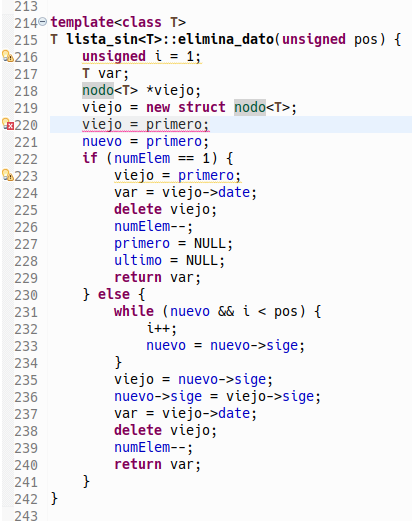
\includegraphics[scale=0.7]{img/captura45.png}
				\caption{Captura de pantalla de la función elimina\_dato}
				\label{captura45}
			\end{figure}
		
			\paragraph{}Este error se materializa de manera idéntica que al anterior error: Primero, la variable \textit{viejo} (puntero) se declara en la línea 218. A continuación, en la línea 219 se reserva memoria para una nueva instancia de la estructura \textit{nodo}. En la línea 220 se le asigna a la variable \textit{viejo} la dirección de memoria del atributo de clase \textit{primero}, generándose en este momento la pérdida de memoria al no haber liberado la memoria a la que se apuntaba anteriormente.
			
			\begin{figure}[H]
				\centering
				
\includegraphics[scale=0.38]{img/captura46.png}
				\caption{Detalle del mensaje de error de cppcheck}
				\label{captura46}
			\end{figure}
	
		\subsubsection{Corrección realizada para solventar el error}
		
			\paragraph{}Para solucionar este error simplemente deberemos eliminar la línea 219 de la función. De esta manera, declaramos la variable \textit{viejo} y justo a continuación le asignamos la dirección de memoria del atributo de clase \textit{primero}. De esta manera el mensaje de pérdida de memoria habrá desaparecido:
	
			\begin{figure}[H]
				\centering
				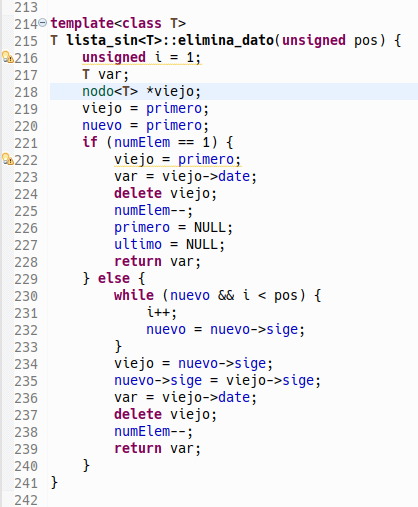
\includegraphics[scale=0.7]{img/captura47.png}
				\caption{Captura de pantalla de la función elimina\_dato}
				\label{captura47}
			\end{figure}

\newpage